\section{Compressed Sensing with Coordinate Descent}\label{cd}
The idea behind compressed sensing is we use prior information about the image, and find the most likely image $x$ from all possible solutions. In practice, we formulate a minimization problem with a data and regularization term. The data term forces the image to be as close to the measured Visibilities as possible, and the regularization term tells us how likely the image is to be true. 

The regularization is responsible for an accurate reconstruction. In this work, two regularizations are used. The L1 pixel regularization is used to demonstrate a simple version of the coordinate descent algorithm. For the actual algorithm starlet regularization is used. Starlets have been used as regularization for the LOFAR interferometer\cite{girard2015sparse}, which has been shown to work.

First, let us look at the coordinate descent algorithm in its simplest form, and discuss its properties. we want to minimize the objective \eqref{cd:clean}, where the data term $\left \| V - F^{-1}x \right \|_2^2$ forces the image to be close to the Visibilities $V$, and the regularization term $\left \| x \right \|_1$ forces the image to have as few non-zero pixels as possible. The parameter $\lambda$ represents our trade-off between reconstruction accuracy and regularization. 
 
\begin{equation}\label{cd:clean}
	\underset{x}{minimize} \: \left \| V - F^{-1}x \right \|_2^2 + \lambda \left \| x \right \|_1 \\
\end{equation}

The objective function \eqref{cd:clean} has a property, which we can exploit with Coordinate Descent: The optimum for a single pixel, if we keep all others fixed, turns out to be a parabola. The optimum for a single pixel of \eqref{cd:clean} is simply finding the apex of a parabola, followed by a shrink operation\footnote{The shrink operation reduces the magnitude of the pixel by $\lambda$. For example: Pixel $x = -12.4$, $\lambda = 0.6$. The new pixel value after shrinkage follows as $shrink(-12.4, 0.6) = -11.9$}. Sadly, the pixels are not independent of each other, and we need multiple iterations over all pixels to converge. This leads to the following reconstruction algorithm, written in python code:

\begin{lstlisting} 
def coordinate_descent(V_residual, x, lambda, max_iter):
	for k in range(0, max_iter):
		for i in pixels_row:
			for j in pixels_column:
				x_old = x[i, j]
				fourier_column = calculate_fourier_transform(i, j)
				fr = real(fourier_column)
				fi = imag(fourier_column)
				rr = real(V_residual)
				ri = imag(V_residual)
				
				#find apex
				a = sum(fr**2 + 2*fr*fi + fi**2)
				b = sum(fr*rr + fr*ri + fi*rr + fi*ri)
				x_new = b / a + x_old
				
				x_new = shrink(x_new, lambda)
				x[i, j] = x_new
				V_residual = V_residual - fourier_column * (x_new - x_old)
\end{lstlisting}\label{cd:basic}

The simple version of coordinate descent converges to a solution which is similar to CLEAN. The convergence rate of coordinate descent is not well understood. Our image reconstruction problem falls in the class of quadratic programming, in coordinate descent converges at least linearly\cite{luo1992convergence}. In practice, the convergence rate can be sped up with heuristics like active set\cite{activeset} and $\lambda$\cite{lambda}. Furthermore, coordinate descent is robust, even when the residual vector is only approximated, which is useful for distributing the algorithm.

The simple approach calculates the whole Fourier Transform Matrix $F^{-1}$ explicitly. The upside is that we do an exact $w$-term correction. The downside is $F^{-1}$ is too large to keep in memory, and too expensive to calculate on the fly for the scale of MeerKAT reconstructions. 

The starlet transform is used from here on. Instead of reconstructing the image directly, we represent the image as a combination of starlets $x = D\alpha$. Where $D$ is an over-complete dictionary of starlets is the starlet component vector. Since the dictionary $D$ is over-complete, it is a matrix with more columns than rows, and does generally not have an inverse  $D^{-1}x \neq \alpha$. However, the starlet transform does have an pseudo-inverse. In this work, the pseudo inverse is used to only look at a subset of starlets, which is likely to be non-zero.




The new objective \eqref{cd:starletobjective} tries to find th

\begin{equation}\label{cd:starletobjective}
\underset{\alpha}{minimize} \: \left \| V - F^{-1}D\alpha \right \|_2^2 + \lambda \left \| \alpha \right \|_1 \\
\end{equation}

Starlet transform can be used to estimate the component vector
parabola for each starlet.






\subsection{Starlet Transform} \label{cd:starlets}

\begin{figure}[h]
	\centering
	\begin{subfigure}[b]{0.4\linewidth}
		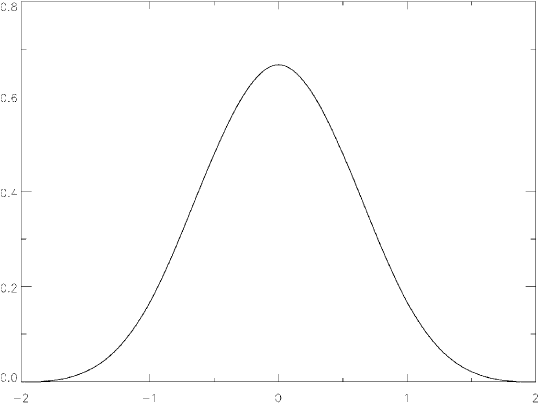
\includegraphics[width=\linewidth]{./chapters/05.algorithms/starlets/scaling.png}
		\caption{Scaling function}
		\label{cd:starlets:scaling}
	\end{subfigure}
	\begin{subfigure}[b]{0.4\linewidth}
		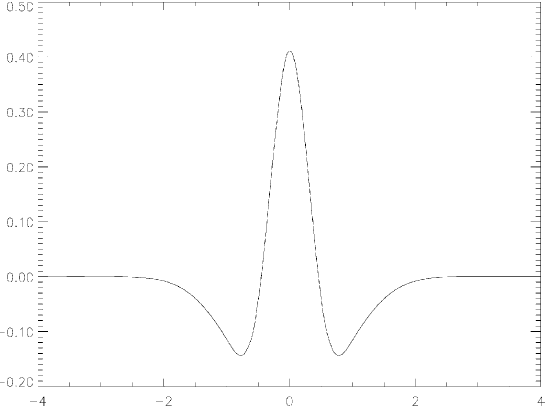
\includegraphics[width=\linewidth]{./chapters/05.algorithms/starlets/wavelet.png}
		\caption{Wavelet function}
		\label{cd:starlets:wavelet}
	\end{subfigure}
	\caption{Scaling and wvelet function of the starlet wavelet. Source: \cite{starck2015starlet}}
	\label{cd:starlets:figure}
\end{figure}

Starlet is a wavelet


Starlet is a multi-scale wavelet representation which were specifically developed for astronomy.

Over-complete representation. More starlets than there are pixels. Sparse representation, the number of non-zero starlets is smaller than the number of pixels


Starlets as a series of convolutions.

Forward transform, from image to starlets

From Starlets to image

\subsection{Active set heuristic with Starlets}\label{cd:heuristic}
Even though the starlets are an over-complete dictionary, they have an approximate transform from image to starlet space. For Coordinate Descent, this can be used as a active set heuristic: We try to find the coefficients which are likely to be non-zero. This helps us so we do not need to calculate the whole matrix product $F^{-1}D$. We only use columns that are likely to be not zero.

\begin{figure}[h]
	\centering
	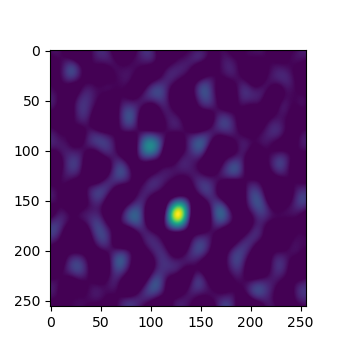
\includegraphics[width=0.5\linewidth]{./chapters/05.algorithms/sim02/starlets0.png}
	\caption{Starlet Level 0}
	\label{alg:heuristic:starlet}
\end{figure}

The higher the number, the more likely this component is to be non-zero. It is essentially a probability distribution for which starlet components are non-zero.

Stupid approach with line search. Could be done more efficiently by using the histogram of the starlet level.

\subsection{Implementation}

\begin{equation}\label{cd:starlet}
\underset{\alpha}{minimize} \: \left \| V - F^{-1}D\alpha \right \|_2^2 + \lambda \left \| \alpha \right \|_1 \\
\end{equation}
coordinate descent with active set heuristic

